% $Id$ %
\screenshot{configure_rockbox/images/ss-sound-settings}{The sound settings screen}{}

The sound settings menu offers a selection of sound settings you may 
change to customise your listening experience.

\section{\label{ref:volume}Volume}
  This setting adjusts the volume of your music. Like most professional
  audio gear and many consumer audio products, Rockbox uses a decibel scale
  where 0~dB is a reference that indicates the maximum volume that the \dap{}
  can produce without possible distortion (clipping). All values lower than
  this reference will be negative and yield a progressively softer volume.
  \nopt{iriverh100,iriverh300,ondavx777}{%
      Values higher than 0~dB are available and can be used to raise the
      volume more than would otherwise be possible. These volume levels will
      ordinarily lead to distorted sound, but might work nicely for music that has
      an otherwise low volume level.
  }
  The volume can be adjusted from a
  \opt{player}{minimum of -78~dB to a maximum of +18~dB.}%
  \opt{recorder,recorderv2fm,ondio}{minimum of -100~dB to a maximum of +12~dB.}%
  \opt{iriverh100,iriverh300}{minimum of -84~dB to a maximum of 0~dB.}%
  \opt{iaudiom3,iaudiom5,iaudiox5,ipod3g,ipod4g,gigabeatf,mrobe100,mpiohd200}{%
      minimum of -73~dB to a maximum of +6~dB.}%
  \opt{ipodnano}{minimum of -72~dB to a maximum of +6~dB.}%
  \opt{ipodvideo,cowond2}{minimum of -89~dB to a maximum of +6~dB.}%
  \opt{ipodnano2g,ipodcolor,ipod1g2g,iriverh10,iriverh10_5gb,sansa,sansaAMS}{minimum of 
      -74~dB to a maximum of +6~dB.}%
  \opt{gigabeats}{minimum of -90~dB to a maximum of +6~dB.}%
  \opt{gigabeatf,vibe500}{minimum of -74~dB to a maximum of +6~dB.}%
  \opt{fuzeplus}{minimum of -100~dB to a maximum of +6~dB.}
  \opt{samsungyh}{minimum of -128~dB to a maximum of 0~dB.}
  \opt{ipodvideo}{\\Remark: Lowering the volume below -57~dB will also affect the line-out 
  and the recording gain.}
  \opt{cowond2}{\\Remark: Lowering the volume below -57~dB will also affect the line-out.}

\nopt{gigabeats}{  
\section{Bass}
  This setting emphasises
  \nopt{iriverh100,iriverh300}{or suppresses}
  the lower (bass) frequencies in the sound. A value of 0~dB means that bass
  sounds are unaltered (flat response).
  \opt{masd}{The minimum setting is -15~dB and the maximum is 15~dB.}%
  \opt{masf}{The minimum setting is -12~dB and the maximum is 12~dB.}%
  \opt{iriverh100,iriverh300}{The minimum setting is 0~dB and the maximum is 24~dB.}%
  \opt{ipodnano,ipodnano2g,ipodcolor,mpiohd200}{%
      The minimum setting is -6~dB and the maximum is 9~dB.}%
  \opt{ipodvideo}{The minimum setting is -12~dB and the maximum is 12~dB.}%
  \opt{iaudiom3,iaudiom5,iaudiox5,sansa,sansaAMS,iriverh10,iriverh10_5gb,vibe500,fuzeplus%
      ,samsungyh}{The minimum setting is -24~dB and the maximum is 24~dB.}

\section{\label{ref:volume_limit}Volume Limit}
  This setting adjusts the maximum volume of your music. The setting is by
  default set to the maximum volume which equals to no limit. To set a volume
  limit, select a volume from the list and the maximum volume will be limited to
  the selected value all over the system.

\opt{ipodvideo}{
\section{Bass Cutoff}
  This setting controls the frequency below which the bass adjustment applies.
  The setting has a range from 1 to 4, where a bigger number affects a bigger
  range of bass frequencies. The actual cutoff frequency used for each setting
  value will vary with sample rate.
}

\section{Treble}
  This setting emphasises
  \nopt{iriverh100,iriverh300}{or suppresses}
  the higher (treble) frequencies in the sound. A value of 0~dB means that
  treble sounds are unaltered (flat response).
  \opt{masd}{The minimum setting is -15~dB and the maximum is 15~dB.}%
  \opt{masf}{The minimum setting is -12~dB and the maximum is 12~dB.}%
  \opt{iriverh100,iriverh300}{The minimum setting is 0~dB and the maximum is 6~dB.}%
  \opt{ipodnano,ipodnano2g,ipodcolor,mpiohd200}{%
      The minimum setting is -6~dB and the maximum is 9~dB.}%
  \opt{ipodvideo}{The minimum setting is -12~dB and the maximum is 12~dB.}%
  \opt{iaudiom3,iaudiom5,iaudiox5,sansa,sansaAMS,iriverh10,iriverh10_5gb,vibe500,fuzeplus%
      ,samsungyh}{The minimum setting is -24~dB and the maximum is 24~dB.}

\opt{ipodvideo}{
\section{Treble Cutoff}
  This setting controls the frequency above which the treble adjustment applies.
  The setting has a range from 1 to 4, where a bigger number affects a smaller
  range of treble frequencies. The actual cutoff frequency used for each setting
  value will vary with sample rate.
}
}

\opt{gigabeats}{
\section{Tone Controls}
  There is a five-band equalizer built into your \dap{} that allows you to
  control various different parameters for each band.  This equalizer is
  implemented in hardware, and therefore does not tax the processor when in use.
  Rockbox also features a more advanced five-band equalizer (see
  \reference{ref:EQ}) that is implemented in software and allows more fine
  grained control, but also requires more processor time. 

  \begin{description}
  \item[Band 1 Gain.]
        This band acts as a low shelf filter that boosts or lowers all
        frequencies below a certain frequency limit, much as a ``bass''
        control found on ordinary stereo systems does. The ``gain'' parameter
        controls how much the loudness of the band is adjusted. Positive
        numbers make the EQ band louder, while negative numbers make that EQ
        band quieter.
  \item[Bands 2-4 Gain.]
        These bands act as peaking filters that boost or lower a frequency
        range centered at a certain frequency. Graphic equalizers in home
        stereos are usually peaking filters. The ``gain'' parameter controls
        how much each band is adjusted as with the the low shelf filter.
  \item[Band 5 Gain.]
        Band 5 acts as a high shelf filter, boosting or lowering all
        frequencies above a certain frequency limit, much like a ``treble''
        control found on ordinary stereo systems does. As with the other bands,
        ``gain'' controls how much each band is adjusted.
  \item[Advanced Tone Control Settings.]
        This submenu allows you to change advanced parameters for each band.
  \end{description}
  
  As a general guide, EQ band 1 should be used for low frequencies, EQ bands 2
  to 4 should be used for mids, and EQ band 5 should be used for highs.\\*

  \subsection{Advanced Tone Control Settings}
    As in the previous menu, the ``gain'' setting controls how much the
    loudness of the band is adjusted.  In addition the following parameters
    can be adjusted:  

  \begin{description}
    \item[Band 1 Frequency.]
        The ``frequency'' parameter sets where the shelving starts to take
        effect. For example, a cutoff frequency of 80~Hz will adjust only very
        low frequencies. A cutoff frequency of 175~Hz, on the other hand, will
        adjust a much wider range of bass frequencies.
  \item[Bands 2-4 Frequency.]
        The ``frequency'' parameter for these bands sets the centre frequency of
        the range that is affected by the gain set.
  \item[Bands 2-4 Width.]
        This parameter sets the width of the range around the centre frequency
        that is affected by the tone control. The possible settings are
        ``wide'' or ``narrow''.
  \item[Band 5 Frequency.]
        This works just as for band 1 frequency, except that it affects the
        high frequency end of the spectrum instead of the low.
  \end{description}

}

\section{Balance}
  This setting controls the balance between the left and right channels. The
  default, 0, means that the left and right outputs are equal in volume.
  Negative numbers increase the volume of the left channel relative to the
  right, positive numbers increase the volume of the right channel relative
  to the left.

\section{Channels}
  A stereo audio signal consists of two channels, left and right. The
  \setting{Channels} setting determines if these channels are to be combined in
  any way, and if so, in what manner they will be combined.
  Available options are:
  %
  \begin{description}
      \item[Stereo.]
          Leave the audio signal unmodified.
      \item[Mono.]
          Combine both channels and send the resulting signal to both stereo
          channels, resulting in a monophonic output.
      \item[Custom.]
          Allows you to manually specify a stereo width with the
          \setting{Stereo Width} setting described later in this chapter.
      \item[Mono Left.]
          Plays the left channel in both stereo channels.
      \item[Mono Right.]
          Plays the right channel in both stereo channels.
      \item[Karaoke.]
          Removes all sound that is common to both channels. Since most
          music is recorded with vocals being equally present in both channels
          to make the singer sound centrally placed, this often (but not 
          always) has the effect of removing the voice track from a song. This 
          setting also very often has other undesirable effects on the sound.
  \end{description}

\section{Stereo Width}
  Stereo width allows you to manually specify the effect that is applied
  when the \setting{Channels} setting is set to ``custom''.
  All values below 100\% will progressively mix the contents of one channel
  into the other. This has the effect of gradually centering the stereo image,
  until you have monophonic sound at 0\%. Values above 100\% will progressively
  remove components in one channel that is also present in the other. This has
  the effect of widening the stereo field. A value of 100\% will leave the
  stereo field unaltered.

\opt{masf}{
  \section{Loudness}
  When listening at low volumes, the ear will tend to make bass and treble
  frequencies sound quieter than they really are. To compensate for this, 
  \setting{Loudness} is an effect which emphasises bass and treble in a fashion
  suited to the human ear. Frequencies in the vocal range are unaffected, since
  the human ear picks these up very easily at any sound level.
  It is of course also possible to use this effect at higher volumes for 
  enhanced bass and treble.
}
  
\opt{masf}{
\section{Auto Volume}
  Auto volume is a feature that automatically lowers the volume on loud parts,
  and then slowly restores the volume to the previous level over a time
  interval. This setting allows this time interval to be configured. Short
  values like 20~ms are useful for ensuring a constant volume for in-car use and
  other applications where background noise makes a constant loudness desirable.
  A longer timeout means that the change in volume back to the previous level
  will be smoother, so there will be fewer sharp changes in volume level.
}

\opt{masf}{
\section{Super Bass}
  This setting changes the threshold at which bass frequencies are affected by
  the \setting{Loudness} setting, making the sound of drums and bass guitar
  louder in comparison to the rest of the sound.  This setting only has an
  effect if \setting{Loudness} is set to a value larger than 0~dB.
}

\opt{masf}{
\section{MDB {}-- Micronas Dynamic Bass}
  The rest of the parameters in this menu relate to the Micronas Dynamic
  Bass (MDB) function. MDB is designed to enable the user to hear bass
  notes that the headphones and/or speakers are not capable of reproducing.
  Every tone has a fundamental frequency (the ``main tone'') and also several
  harmonics, which are related to that tone. The human brain has a mechanism
  whereby it can actually infer the presence of bass notes from the higher
  harmonics that they would generate.

  The practical upshot of this is that MDB produces a more authentic sounding
  bass by tricking the brain into believing it is hearing tones that the 
  headphones or speakers are not capable of reproducing.

  The MDB parameters are as follows:
  %
  \begin{description}
  \item[MDB enable.]
    This turns the MDB feature on or off. For many users this will be the
    only setting they need, since Rockbox picks sensible defaults for the
    other parameters. MDB is turned off by default.
  \item[MDB strength.]
    How loud the harmonics generated by MDB will be.
  \item[MDB Harmonics.]
    The percentage of the low notes that is converted into harmonics.
    If low notes are causing speaker distortion, this can be set to 100\%
    to eliminate the fundamental completely and only produce harmonics in the
    signal. If set to 0\% this is the same as turning the MDB feature off.
  \item[MDB Centre Frequency.]
    The cutoff frequency of your headphones or speakers. This is usually
    given in the specification for the headphones/speakers.
  \item[MDB shape.]
    It is recommended that this parameter be set to 1.5 times the centre frequency.

    This is the frequency up to which harmonics are generated. Some of the
    lower fundamentals near the cut{}-off range will have their lower
    harmonics cut, since they will be below the range of the speakers.
    Fundamentals between the cut{}-off frequency and the lower frequency
    will have their harmonics proportionally boosted to compensate and restore
    the `loudness' of these notes.

    For most users, the defaults should provide an improvement in sound
    quality and can be safely left as they are. For reference, the defaults
    Rockbox uses are:
    %
    \begin{table}[h!]
       \begin{rbtabular}{0.5\textwidth}{Xc}{Setting & Value}{}{}
          MDB Strength & 50~dB \\
          MDB Harmonics & 48\% \\
          MDB Centre Frequency & 60~Hz \\
          MDB Shape & 90~Hz \\
       \end{rbtabular}
    \end{table}
      
  \end{description}
}

\opt{swcodec}{
\section{Crossfeed}
  Crossfeed attempts to make the experience of listening to music on
  headphones more similar to listening to music with stereo speakers. When you
  listen to music through speakers, each ear will hear sound originating from
  both speakers. However, the sound from the left speaker reaches your right
  ear slightly later than it does your left ear, and vice versa.\\

  The human ear and brain together are very good at interpreting the time
  differences between direct sounds and reflected sounds and using that
  information to identify the direction that the sound is coming from. On the
  other hand, when listening to headphones, each ear hears only the stereo
  channel corresponding to it. The left ear hears only the left channel and
  the right ear hears only the right channel. The result is that sound from
  headphones does not provide the same spatial cues to your ear and brain as
  speakers, and might for that reason sound unnatural to some listeners.\\
    
  The crossfeed function uses an algorithm to feed a delayed and filtered
  portion of the signal from the right channel into the left channel and vice
  versa in order to simulate the spatial cues that the ear and brain receive
  when listening to a set of loudspeakers placed in front of the listener. The
  result is a more natural stereo image that can be especially appreciated in
  older rock and jazz records, where one instrument is often hard-panned to
  just one of the speakers. Many people will find such records tiring to listen
  to using earphones and no crossfeed effect.\\

  Crossfeed has the following settings:
  \begin{description}
  \item[Crossfeed.]
    Selects whether the crossfeed effect is to be enabled or not.
  \item[Direct Gain.]
    How much the level of the audio that travels the direct path from a speaker
    to the corresponding ear is supposed to be decreased.
  \item[Cross Gain.]
    How much the level of the audio that travels the cross path from a speaker
    to the opposite ear is to be decreased.
  \item[High-Frequency Attenuation.]
    How much the upper frequencies of the cross path audio will be dampened.
    Note that the total level of the higher frequencies will be a combination
    of both this setting and the \setting{Cross Gain} setting.
  \item[High-Frequency Cutoff.]
    Decides at which frequency the cross path audio will start to be cut
    by the amount described by the \setting{High-Frequency Attenuation} 
    setting.
  \end{description}

  Most users will find the default settings to yield satisfactory results, but
  for the more adventurous user the settings can be fine-tuned to provide a
  virtual speaker placement suited to ones preference.
  % TODO: adapt the guidelines for crossfeed settings found here?
  % http://www.ohl.to/interests-in-audio/crossfeed-and-eq-for-headphones/ 
  Beware that the crossfeed function is capable of making the audio distort
  if you choose settings which result in a too high output level.
}
  
\opt{swcodec}{
\section{\label{ref:EQ}Equalizer}
  \screenshot{configure_rockbox/images/ss-equalizer}{The graphical equalizer}{}
  Rockbox features a parametric equalizer (EQ). In contrast to non-parametric
  equalizers, a parametric EQ enables adjusting the center frequency, gain, and
  width of EQ bands separately.  The ability to adjust the frequency and width
  of bands enables more precise control of the EQ frequency response while 
  avoiding the use of a large number of bands (often 12+) needed in a 
  non-parametric EQ.
  
  The graphic below illustrates how the width of 10kHz band can be adjusted to
  cover a wider (lower Q) or narrower (higher Q) range of frequencies.
  
  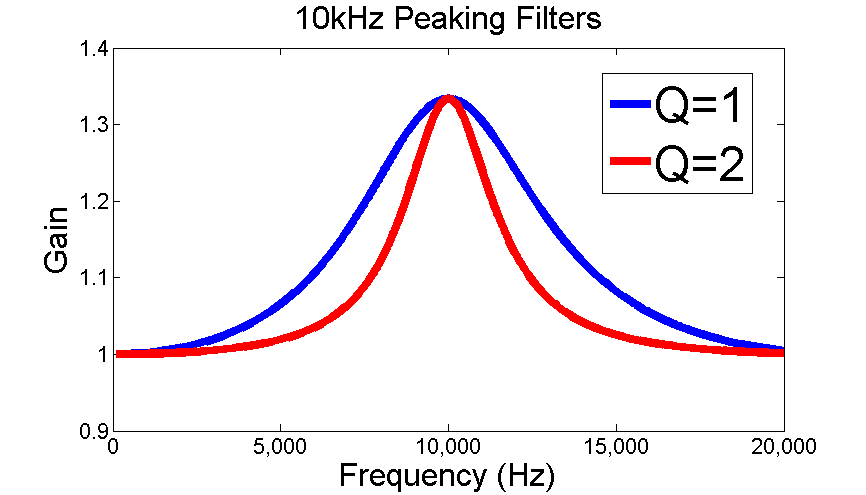
\includegraphics[width=14cm]{configure_rockbox/images/Q_factor.png}
  
  \nopt{gigabeats}{In some ways the EQ is similar to the
  \setting{Bass} and \setting{Treble} settings described earlier, but the EQ
  allows you to control the sound much more carefully.  Note that the parameteric
  EQ bands will be applied in addition to any bass or treble tone controls. 
  } \opt{gigabeats}{The EQ  is similar to the \setting{Tone Controls} described 
  above, but allows more delicate control.}\\
  
  \note{A maximum of 10 EQ bands are possible on most devices, but using more
        than are required will waste battery and introduce additional rounding
        noise.  For best results, use the fewest number of bands required.}

  Rockbox's parametric EQ is composed of up to ten different bands:
  \begin{description}
  \item[Band 0: Low shelf filter.]
        The low shelf filter boosts or lowers all frequencies below a certain
        frequency limit, much as the ``bass'' control found on ordinary
        stereo systems does.
        Adjust the ``cutoff'' frequency parameter to decide where the shelving
        starts to take effect. For example, a cutoff frequency of 50~Hz will
        adjust only very low frequencies. A cutoff frequency of 200~Hz, on the
        other hand, will adjust a much wider range of bass frequencies.
        The ``gain'' parameter controls how much the loudness of the band is
        adjusted. Positive numbers make the EQ band louder, while negative
        numbers make that EQ band quieter.
        The ``Q'' parameter should always be set to 0.7 for the shelving
        filters. Higher values will add a small boost around the cutoff
        frequency that is almost always undesirable.
  \item[Bands 1-8: Peaking filters.]
        Peaking EQ filters boost or lower a frequency range centered at the
        centre frequency chosen.
        Graphic equalizers in home stereos are usually peaking
        filters. The peaking filters in Rockbox's EQ lets you adjust three
        different parameters for EQ bands 1 through 8. The ``centre'' parameter
        controls the centre frequency of the frequency range that is affected
        as described above.
        The ``gain'' parameter controls how much each band is adjusted, and
        works as for the low shelf filter.
        Finally, the ``Q'' parameter controls how wide or narrow the affected
        frequency range is. Higher Q values will affect a narrower band of
        frequencies, while lower Q values will affect a wider band of
        frequencies.
  \item[Band 9: High shelf filter.]
        A high shelf filter boosts or lowers all frequencies above a certain
        frequency limit, much as the ``treble'' control found on ordinary
        stereo systems does.
        The high shelf filter is adjusted the same way as the low shelf filter,
        except that it works on the high end of the frequency spectrum rather
        than the low end.
  \end{description}
  As a general guide, EQ band 0 should be used for low frequencies, EQ bands 1
  through 8 should be used for mids, and EQ band 9 should be used for highs.

\begin {description}
  \item[Enable EQ.]
  This option controls whether the EQ is on or off.

  \item[Graphical EQ.]
  This option brings up a graphic EQ screen, which allows adjustment of each of
  the three parameters described above (gain, centre frequency, and Q) for each
  of the five EQ bands.
  
    \begin{btnmap}
      \opt{IRIVER_H100_PAD,IRIVER_H300_PAD,IAUDIO_X5_PAD,GIGABEAT_PAD%
          ,GIGABEAT_S_PAD,SANSA_C200_PAD,IAUDIO_M3_PAD,MROBE100_PAD%
          ,SANSA_CLIP_PAD,SANSA_FUZEPLUS_PAD,SAMSUNG_YH92X_PAD}{\ButtonRight}
      \opt{SANSA_E200_PAD,SANSA_FUZE_PAD,IPOD_4G_PAD,IPOD_3G_PAD}{\ButtonScrollFwd}
      \opt{IRIVER_H10_PAD}{\ButtonScrollUp}
      \opt{PBELL_VIBE500_PAD}{\ButtonUp}
      \opt{MPIO_HD200_PAD}{\ButtonVolUp}
      \opt{MPIO_HD300_PAD}{\ButtonScrollUp}
      \opt{touchscreen}{\TouchMidRight}
          &
      \opt{HAVEREMOTEKEYMAP}{
          \opt{GIGABEAT_RC_PAD}{\ButtonRCFF}
          \opt{IAUDIO_RC_PAD}{\ButtonRCRight}
          &}
      Raises the highlighted parameter.
          \\
      %
      \opt{IRIVER_H100_PAD,IRIVER_H300_PAD,IAUDIO_X5_PAD,GIGABEAT_PAD%
          ,GIGABEAT_S_PAD,SANSA_C200_PAD,IAUDIO_M3_PAD,MROBE100_PAD%
          ,SANSA_CLIP_PAD,SANSA_FUZEPLUS_PAD,SAMSUNG_YH92X_PAD}{\ButtonLeft}
      \opt{SANSA_E200_PAD,SANSA_FUZE_PAD,IPOD_4G_PAD,IPOD_3G_PAD}{\ButtonScrollBack}
      \opt{IRIVER_H10_PAD}{\ButtonScrollDown}
      \opt{PBELL_VIBE500_PAD}{\ButtonDown}
      \opt{MPIO_HD200_PAD}{\ButtonVolDown}
      \opt{MPIO_HD300_PAD}{\ButtonScrollDown}
      \opt{touchscreen}{\TouchMidLeft}
          &
      \opt{HAVEREMOTEKEYMAP}{
          \opt{GIGABEAT_RC_PAD}{\ButtonRCRew}
          \opt{IAUDIO_RC_PAD}{\ButtonRCLeft}
          &}
      Lowers the highlighted parameter.
          \\
      %
      \opt{IPOD_4G_PAD,IPOD_3G_PAD,PBELL_VIBE500_PAD}{\ButtonLeft}
      \opt{IRIVER_H100_PAD,IRIVER_H300_PAD,IAUDIO_X5_PAD,SANSA_E200_PAD,SANSA_C200_PAD%
          ,SANSA_FUZE_PAD,GIGABEAT_PAD,GIGABEAT_S_PAD,IAUDIO_M3_PAD,MROBE100_PAD%
          ,SANSA_CLIP_PAD,SANSA_FUZEPLUS_PAD,SAMSUNG_YH92X_PAD}{\ButtonUp}
      \opt{IRIVER_H10_PAD,MPIO_HD200_PAD,MPIO_HD300_PAD}{\ButtonRew}
      \opt{touchscreen}{\ActionStdPrev}
          &
      \opt{HAVEREMOTEKEYMAP}{
          \opt{IRIVER_RC_H100_PAD}{\ButtonRCRew}
          \opt{GIGABEAT_RC_PAD}{\ButtonRCVolUp}
          \opt{IAUDIO_RC_PAD}{\ButtonRCUp}
          &}
      Moves to the previous EQ band.
          \\
      %
      \opt{IPOD_4G_PAD,IPOD_3G_PAD,PBELL_VIBE500_PAD}{\ButtonRight}
      \opt{IRIVER_H100_PAD,IRIVER_H300_PAD,IAUDIO_X5_PAD,SANSA_E200_PAD,SANSA_C200_PAD%
          ,SANSA_FUZE_PAD,GIGABEAT_PAD,GIGABEAT_S_PAD,IAUDIO_M3_PAD,MROBE100_PAD%
          ,SANSA_CLIP_PAD,SANSA_FUZEPLUS_PAD,SAMSUNG_YH92X_PAD}{\ButtonDown}
      \opt{IRIVER_H10_PAD,MPIO_HD200_PAD,MPIO_HD300_PAD}{\ButtonFF}
      \opt{touchscreen}{\ActionStdNext}
          &
      \opt{HAVEREMOTEKEYMAP}{
          \opt{IRIVER_RC_H100_PAD}{\ButtonRCFF}
          \opt{GIGABEAT_RC_PAD}{\ButtonRCVolDown}
          \opt{IAUDIO_RC_PAD}{\ButtonRCDown}
          &}
      Moves to the next EQ band.
          \\
      %
      \opt{IRIVER_H100_PAD,IRIVER_H300_PAD,GIGABEAT_PAD,GIGABEAT_S_PAD,IAUDIO_X5_PAD%
          ,SANSA_C200_PAD,IPOD_4G_PAD,IPOD_3G_PAD,IPOD_VIDEO_PAD,SANSA_E200_PAD%
          ,SANSA_FUZE_PAD,MROBE100_PAD,SANSA_CLIP_PAD,SANSA_FUZEPLUS_PAD}{\ButtonSelect}
      \opt{MPIO_HD200_PAD}{\ButtonFunc}
      \opt{MPIO_HD300_PAD}{\ButtonEnter}
      \opt{PBELL_VIBE500_PAD}{\ButtonOK}
      \opt{IRIVER_H10_PAD}{\ButtonRight}
      \opt{IAUDIO_M3_PAD}{\ButtonPlay}
      \opt{SAMSUNG_YH92X_PAD}{\ButtonFF}
      \opt{touchscreen}{\TouchCenter
          \opt{COWON_D2_PAD}{/ \ButtonMenu}}
          &
      \opt{HAVEREMOTEKEYMAP}{     
          \opt{IRIVER_RC_H100_PAD}{\ButtonRCSelect}
          \opt{GIGABEAT_RC_PAD,IAUDIO_RC_PAD}{\ButtonRCPlay}
          &}
      Toggles the cursor among the three parameters (gain, centre frequency,
      Q) for the selected EQ band
          \\
      %
      \opt{IRIVER_H100_PAD,IRIVER_H300_PAD}{\ButtonMode}
      \opt{IPOD_4G_PAD,IPOD_3G_PAD,MPIO_HD300_PAD}{\ButtonMenu}
      \opt{IAUDIO_X5_PAD}{\ButtonPower/\ButtonRec}
      \opt{IAUDIO_M3_PAD,MPIO_HD200_PAD}{\ButtonRec}
      \opt{SANSA_E200_PAD,SANSA_FUZE_PAD,IRIVER_H10_PAD}{\ButtonLeft}
      \opt{GIGABEAT_PAD,GIGABEAT_S_PAD,SANSA_C200_PAD,MROBE100_PAD,SANSA_CLIP_PAD}{\ButtonPower}
      \opt{PBELL_VIBE500_PAD}{\ButtonCancel}
      \opt{SANSA_FUZEPLUS_PAD}{\ButtonBack}
      \opt{SAMSUNG_YH92X_PAD}{\ButtonRew}
      \opt{touchscreen}{\TouchTopLeft
          \opt{COWON_D2_PAD}{/ \ButtonPower}}
          &
      \opt{HAVEREMOTEKEYMAP}{ 
          \opt{IRIVER_RC_H100_PAD}{\ButtonRCStop}
          \opt{GIGABEAT_RC_PAD}{\ButtonRCDsp}
          \opt{IAUDIO_RC_PAD}{\ButtonRCRec}
          &}
      Exits the graphic EQ screen.
          \\
    \end{btnmap}

  \item[Pre-cut.]
  If too much positive gain is added through the graphical EQ, your music may 
  distort.  The \setting{Precut} setting allows you to apply a global negative
  gain to decoded audio, cancelling out positive gain from the EQ.  This will
  prevent distortion when boosting certain frequency ranges, at the expense of 
  making audio quieter.
  
  Alternatively, precut can be used with a flat EQ curve to implement a volume
  cap.  For example, on a player that allows overdriving the headphone output
  to +6dB, maximum volume can be capped to +0dB by applying 6dB of precut. Note
  that precut is not applied if EQ is disabled.  

\item[Simple EQ.]
This option provides an easier alternative for those who are daunted by all of
the parameters that can be adjusted using the graphical EQ. With the
\setting{Simple EQ}, the only parameter that can be adjusted is the gain.

\item[Advanced EQ.]
This sub menu provides options for adjusting the same parameters as the
\setting{Graphical EQ}. The only difference is that the parameters are
adjusted through textual menus rather than through a graphic interface.

\item[Save EQ Preset.]
This option saves the current EQ configuration in a \fname{.cfg} file.

\item[Browse EQ Presets.]
This menu displays a list of EQ presets, as well as any EQ configurations saved
using the \setting{Save EQ Preset} option. Users unfamiliar with the
operation of a parametric EQ may wish to use the presets instead of trying to
configure the EQ, or use the presets for designing their own custom EQ
settings.

\end{description}
}

\opt{swcodec}{
\section{Dithering}
This setting controls the dithering and noise shaping functionality of Rockbox.

Most of Rockbox' audio file decoders work at a higher bit depth than the 16 bits
used for output on the \daps{} audio connectors. The simplest way to
convert from one bit depth to another is simply discarding all the surplus bits.
This is the default behaviour, and adds distortion to the signal that will
vary in character along with the desired sound.

Dithering adds low-level noise to the signal prior to throwing away the surplus
bits, which gives the resulting signal a uniform noise floor which is
independent of the signal. Most people find this noise preferable to the
time-varying noise heard when not performing dithering.

After dithering, noise shaping is performed. This basically just pushes the
dithering noise to the parts of the frequency spectrum humans cannot hear so
easily. In Rockbox' case, some of the noise is pushed up to above 10~kHz.

This setting will be put to its best use when listening to dynamic music with
frequently occuring quiet parts, classical music being a typical example. It is
worth noting that the effects of dithering and noise shaping are very subtle,
and not easily noticable.

Rockbox uses highpass triangular distribution noise as the dithering noise
source, and a third order noise shaper.
}

\opt{swcodec}{%
\opt{pitchscreen}{%
\section{Timestretch}
Enabling \setting{Timestretch} allows you to change the playback speed without
it affecting the pitch of the recording. After enabling this feature and
rebooting, you can access this via the \setting{Pitch Screen}. This function is
intended for speech playback and may significantly dilute your listening
experience with more complex audio. See \reference{sec:pitchscreen} for more
details about how to use the feature.
}
}

\opt{swcodec}{
\section{Compressor}
The \setting{Compressor} reduces, or compresses, the dynamic range of the audio
signal.  This makes the quieter and louder sections closer to the same volume
level by progressively reducing the gain of louder signals.  When subsequently
amplified, this has the effect of making the quieter sections louder while
keeping the louder sections from clipping.  This allows listening to the quiet
sections of dynamic material in noisy environments while preventing sudden loud
sections from being overbearing.

There are several settings associated with the compressor.  The first, and most
important, is the \setting{Threshold}.  The threshold is the audio input level
at which the compressor begins to act.  Any level louder than the threshold
will be compressed to some extent.  The maximum amount of compression, or the
quietest level at which the compressor will operate, is -24~dB.  The default of
Off disables the compressor.

The \setting{Makeup Gain} setting has two options: Off and Auto.  Off means
that the compressed audio will not be amplified after compression.  The default
of Auto will amplify the signal so that the loudest possible signal after
compression will be just under the clipping limit.  This is desirable because
the compressed signal without makeup gain is quieter than the input signal.
Makeup Gain in Auto restores the signal to the maximum possible level and
brings the quieter audio up with it.  This is what makes it possible to hear
the quieter audio in noisy environments.

The \setting{Ratio} setting determines how aggressively the compressor reduces
gain above the threshold.  For example, the 2:1 setting means that for each
two decibels of input signal above the threshold, the compressor will only
allow the output to appear as one decibel.  The higher the ratio, the harder
the signal is compressed.  The ratio setting of Limit means essentially a ratio
of infinity to one.  In this case, the output signal is not allowed to exceed
the threshold at all.

The \setting{Knee} setting determines how abrupt the transition is from a
non-compressed signal to a compressed signal.  Hard Knee means that the
transition occurs precisely at the threshold.  The Soft Knee setting smoothes
the transition from plus or minus three decibels around the threshold.

The \setting{Attack Time} setting sets the delay in milliseconds between the
input signal exceeding the activation threshold and acting upon it.

The \setting{Release Time} setting sets the recovery time after the signal is
compressed.  Once the compressor determines that compression is necessary,
the input signal is reduced appropriately, but the gain isn't allowed to
immediately return to normal levels.  This is necessary to reduce artifacts
such as ``pumping.''  Instead, the gain is allowed to return to normal at the
chosen rate.  Release Time is the time for the gain to recover by 10~dB.
}
